%----------------------------------------------------------------------------------------
%	PACKAGES AND OTHER DOCUMENT CONFIGURATIONS
%----------------------------------------------------------------------------------------
\documentclass[10pt, a4paper, twocolumn]{article} % 10pt font size (11 and 12 also possible), A4 paper (letterpaper for US letter) and two column layout (remove for one column)
\linespread{1.1} % Line spacing
%%%%%%%%%%%%%%%%%%%%%%%%%%%%%%%%%%%%%%%%%
% Wenneker Article
% Structure Specification File
% Version 1.0 (28/2/17)
%
% This file originates from:
% http://www.LaTeXTemplates.com
%
% Authors:
% Frits Wenneker
% Vel (vel@LaTeXTemplates.com)
%
% License:
% CC BY-NC-SA 3.0 (http://creativecommons.org/licenses/by-nc-sa/3.0/)
%
%%%%%%%%%%%%%%%%%%%%%%%%%%%%%%%%%%%%%%%%%

%----------------------------------------------------------------------------------------
%	PACKAGES AND OTHER DOCUMENT CONFIGURATIONS
%----------------------------------------------------------------------------------------

\usepackage[english]{babel} % English language hyphenation

\usepackage{microtype} % Better typography

\usepackage{amsmath,amsfonts,amsthm} % Math packages for equations

\usepackage[svgnames]{xcolor} % Enabling colors by their 'svgnames'

\usepackage[hang, small, labelfont=bf, up, textfont=it]{caption} % Custom captions under/above tables and figures

\usepackage{booktabs} % Horizontal rules in tables

\usepackage{lastpage} % Used to determine the number of pages in the document (for "Page X of Total")

\usepackage{graphicx} % Required for adding images

\usepackage{float} % Required for positioning figures and tables

\usepackage{enumitem} % Required for customising lists
\setlist{noitemsep} % Remove spacing between bullet/numbered list elements

\usepackage{sectsty} % Enables custom section titles
\allsectionsfont{\usefont{OT1}{phv}{b}{n}} % Change the font of all section commands (Helvetica)

%----------------------------------------------------------------------------------------
%	MARGINS AND SPACING
%----------------------------------------------------------------------------------------

\usepackage{geometry} % Required for adjusting page dimensions

\geometry{
	top=1cm, % Top margin
	bottom=1.5cm, % Bottom margin
	left=2cm, % Left margin
	right=2cm, % Right margin
	includehead, % Include space for a header
	includefoot, % Include space for a footer
	%showframe, % Uncomment to show how the type block is set on the page
}

\setlength{\columnsep}{7mm} % Column separation width

%----------------------------------------------------------------------------------------
%	FONTS
%----------------------------------------------------------------------------------------

\usepackage[T1]{fontenc} % Output font encoding for international characters
\usepackage[utf8]{inputenc} % Required for inputting international characters

\usepackage{XCharter} % Use the XCharter font

%----------------------------------------------------------------------------------------
%	HEADERS AND FOOTERS
%----------------------------------------------------------------------------------------

\usepackage{fancyhdr} % Needed to define custom headers/footers
\pagestyle{fancy} % Enables the custom headers/footers

\renewcommand{\headrulewidth}{0.0pt} % No header rule
\renewcommand{\footrulewidth}{0.4pt} % Thin footer rule

\renewcommand{\sectionmark}[1]{\markboth{#1}{}} % Removes the section number from the header when \leftmark is used

%\nouppercase\leftmark % Add this to one of the lines below if you want a section title in the header/footer

% Headers
\lhead{} % Left header
\chead{\textit{\thetitle}} % Center header - currently printing the article title
\rhead{} % Right header

% Footers
\lfoot{} % Left footer
\cfoot{} % Center footer
\rfoot{\footnotesize Page \thepage\ of \pageref{LastPage}} % Right footer, "Page 1 of 2"

\fancypagestyle{firstpage}{ % Page style for the first page with the title
	\fancyhf{}
	\renewcommand{\footrulewidth}{0pt} % Suppress footer rule
}

%----------------------------------------------------------------------------------------
%	TITLE SECTION
%----------------------------------------------------------------------------------------

\newcommand{\authorstyle}[1]{{\large\usefont{OT1}{phv}{b}{n}\color{DarkRed}#1}} % Authors style (Helvetica)

\newcommand{\institution}[1]{{\footnotesize\usefont{OT1}{phv}{m}{sl}\color{Black}#1}} % Institutions style (Helvetica)

\usepackage{titling} % Allows custom title configuration

\newcommand{\HorRule}{\color{DarkGoldenrod}\rule{\linewidth}{1pt}} % Defines the gold horizontal rule around the title

\pretitle{
	\vspace{-30pt} % Move the entire title section up
	\HorRule\vspace{10pt} % Horizontal rule before the title
	\fontsize{32}{36}\usefont{OT1}{phv}{b}{n}\selectfont % Helvetica
	\color{DarkRed} % Text colour for the title and author(s)
}

\posttitle{\par\vskip 15pt} % Whitespace under the title

\preauthor{} % Anything that will appear before \author is printed

\postauthor{ % Anything that will appear after \author is printed
	\vspace{10pt} % Space before the rule
	\par\HorRule % Horizontal rule after the title
	\vspace{20pt} % Space after the title section
}

%----------------------------------------------------------------------------------------
%	ABSTRACT
%----------------------------------------------------------------------------------------

\usepackage{lettrine} % Package to accentuate the first letter of the text (lettrine)
\usepackage{fix-cm}	% Fixes the height of the lettrine

\newcommand{\initial}[1]{ % Defines the command and style for the lettrine
	\lettrine[lines=3,findent=4pt,nindent=0pt]{% Lettrine takes up 3 lines, the text to the right of it is indented 4pt and further indenting of lines 2+ is stopped
		\color{DarkGoldenrod}% Lettrine colour
		{#1}% The letter
	}{}%
}

\usepackage{xstring} % Required for string manipulation

\newcommand{\lettrineabstract}[1]{
	\StrLeft{#1}{1}[\firstletter] % Capture the first letter of the abstract for the lettrine
	\initial{\firstletter}\textbf{\StrGobbleLeft{#1}{1}} % Print the abstract with the first letter as a lettrine and the rest in bold
}

%----------------------------------------------------------------------------------------
%	BIBLIOGRAPHY
%----------------------------------------------------------------------------------------

\usepackage[backend=bibtex,style=authoryear,natbib=true]{biblatex} % Use the bibtex backend with the authoryear citation style (which resembles APA)

\addbibresource{example.bib} % The filename of the bibliography

\usepackage[autostyle=true]{csquotes} % Required to generate language-dependent quotes in the bibliography
 % Specifies the document structure and loads requires packages
%----------------------------------------------------------------------------------------
%	ARTICLE INFORMATION
%----------------------------------------------------------------------------------------
\title{Meta Defender} % The article title
\author{
	\authorstyle{alvin@metadefender.finance} % Authors
	\newline
	\authorstyle{angie@metadefender.finance}
	\newline
	\authorstyle{vincent@metadefender.finance}
	\newline\newline % Space before institutions
	%\textsuperscript{1}\institution{Universidad Nacional Autónoma de México, Mexico City, Mexico}\\ % Institution 1
	%\textsuperscript{2}\institution{University of Texas at Austin, Texas, United States of America}\\ % Institution 2
	%\textsuperscript{3}\institution{\texttt{LaTeXTemplates.com}} % Institution 3
}
\date{\today} % Add a date here if you would like one to appear underneath the title block, use \today for the current date, leave empty for no date
%----------------------------------------------------------------------------------------

\begin{document}

\maketitle % Print the title

\thispagestyle{firstpage} % Apply the page style for the first page (no headers and footers)

%----------------------------------------------------------------------------------------
%	ABSTRACT
%----------------------------------------------------------------------------------------

\lettrineabstract{The security industry is enormous and plays an important role in the traditional financial market.
However, the traditional insurance model does not work in the Web3 world because the claiming procedures are time-consuming and opaque.
Furthermore, one cannot enter the insurance industry efficiently because capital for underwriting is only available to the "Big Money".
MetaDefender serves as a pioneer in creating a permissionless platform for risk/insurance trading on-chain, allowing both underwriters and policy buyers to benefit from the blockchain's instant, convenient, and transparent service.
}

%----------------------------------------------------------------------------------------
%	ARTICLE CONTENTS
%----------------------------------------------------------------------------------------

\section{Background}\label{sec:background}
Since DeFi's inception in 2020, more than 5.7 billion dollars\footnote{https://rekt.news/leaderboard/} have been lost due to hacking attacks or contract faults.
Furthermore, the depreciation of LUNA and the collapse of FTX harm the crypto world.
The crypto realm is unmanageable and fascinating, like a wild horse.
The threats we face must not be underestimated.

We are now in the Web3 Age of Discovery, fearless of hardships, fearless of ships that are not strong enough, not technologically advanced enough, but we will always take risks, break away from the stale comfort zone, return to the great seafaring era, write amazing music in the deathly unknown, and establish our own order.


%------------------------------------------------

\section{Introduction}\label{sec:introduction}
In this paper, we present Meta Defender, a novel automated protocol for trading insurance deployed in blockchains.
Prior to the protocols before, we present several advantages:

\begin{itemize}
	\item \textit{Dynamic Pricing Model} : We modified the option pricing model to make it acceptable for buying and selling policies.
	The pricing model will automatically compute the price of each insurance based on the policy's period and coverage.
	\item \textit{EpochManagement in Trading} : The epoch is included to prevent lengthy loops in computation.
	We divided the timeline into discrete epochs so that others might deposit and withdraw independently.
	We can simply compute how much one's asset is locked and how much one receives in incentives using the epoch.
	\item \textit{Rekt affect Token Collection} : Unlike other risk-coverage protocols.
	MetaDefender collects rekt affect tokens from the policyholders to rescue the rekt affect community.
	The toxic assets resulting from DeFi REKT won't simply be cast aside as waste.
	The disposition of these assets and the resultant income streams also provide additional possibility, propelling all participants towards further progress in the realm of Web3.
	Both underwriters and policyholders reap the benefits mentioned above as well as the subsequent DEF rewards.
	With all of these rekt affect tokens locked, we will play a significant part in rescuing the project.
\end{itemize}

%------------------------------------------------

\section{Solution Overview}\label{sec:solution-overview}
The workflow of the underwriting, buying, and settlement process, as well as the claim procedure, is depicted in the two charts below.
Here are the main parts of the system.

\begin{figure}[H]
	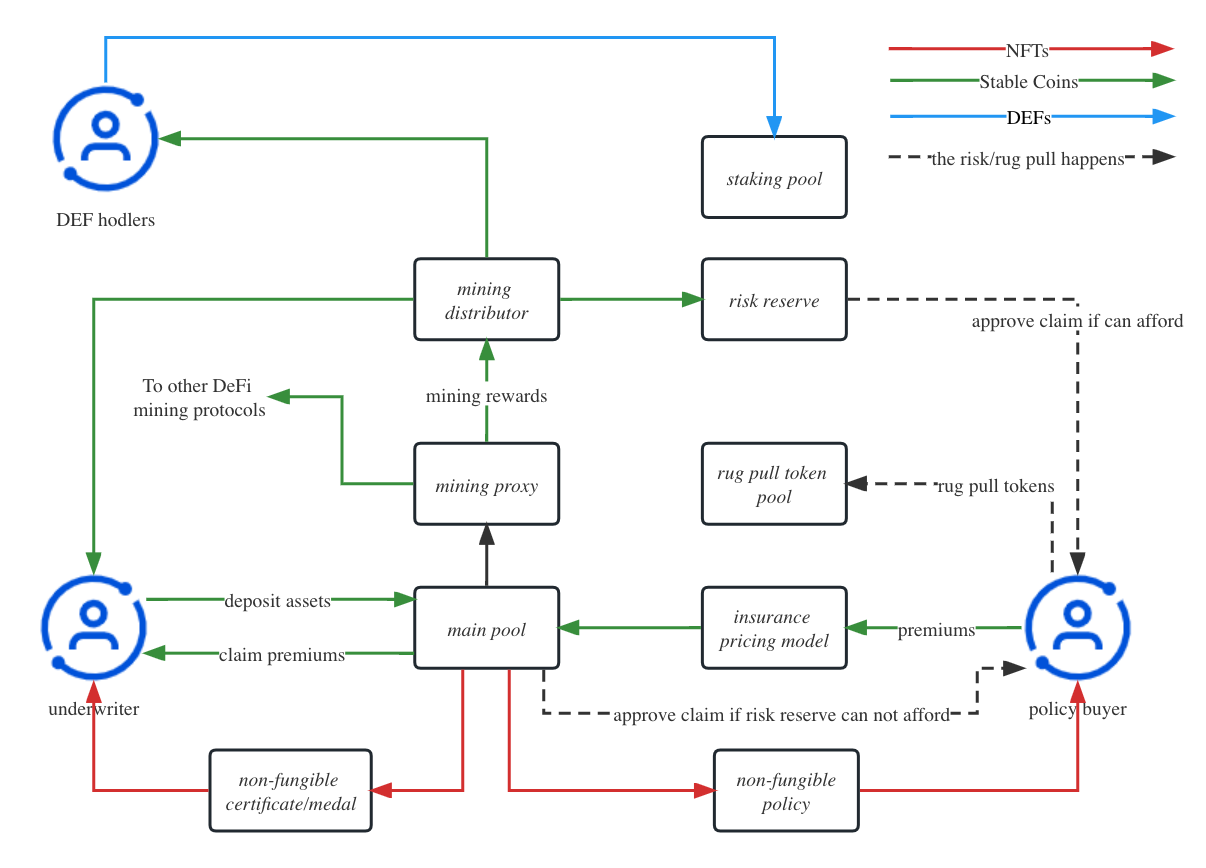
\includegraphics[width=\linewidth]{../workflow_process_on} % Figure image
	\caption{MetaDefender Workflow} % Figure caption
	\label{fig:workflow} % Label for referencing with \ref{bear}
\end{figure}

\begin{itemize}
    \item main pool: The key component of the system.
	The (total value locked)TVL in the pool is made up of three components: the underwriters' assets given, the premium paid by policyholders, and the unfrozen assets temporarily held for some underwriters' early departures.
	\item insurance pricing model: The premium computation portion.
	It employs the American binary option formula to estimate the insurance premium using the policy duration and policy coverage as input parameters.
	\item non-fungible certificate/policy: The NFT is responsible for the liquidity certificate and policy.
	The NFT is coined and transmitted to the user when the user underwrites/purchases insurance.
	The NFT adheres to the ERC721 standard, and users can sell their liquidity at any moment.
	\item risk reserve: Because preserving underwriters' capital SAFU is vital, a portion of the mining rewards will be transferred to the risk reserve pool.
	If the risk situation occurs and policyholders apply for claims, the protocol will initially use the funds in the risk reserve pool rather than the main pool.
	If the funds are inadequate to cover all claims, the main pool will step in to pay the rest of money, putting the underwriters' capital at risk.
	\item DAO: The DAO is made up of numerous stakeholder groups, including the MetaDefender team, insurance specialists, the EVM safety team, and DEF hodlers.
	They vote in the DAO voting system to determine if we will approve the claim after a thorough investigation of the issue.
\end{itemize}


\section{Dynamic Pricing Model}\label{sec:dynamic-pricing-model}
\cite{Marcus et al., 1984} examined the value of FDIC deposit insurance as an option and utilized the option pricing model to calculate the cost of insurance.
Following that, \cite{RONN et al., 1986}, \cite{Laeven et al., 2002}, and \cite{Falkenheim et al., 2003} conducted more study on insurance and option comparisons.

The DeFi insurance market, like the traditional insurance market, will pay either a defined amount of money known as policy coverage or nothing at all.
If the risk/rekt occurred during the time designated by the policy buyer, the policy buyer will get the claim if the application is granted by the DAO; otherwise, the underwriters will claim the premium and the policy buyer will receive nothing.
This scenario is quite similar to the American binary option.
If the underlying price reaches the strike price before the expiration period, the option can be exercised at any moment before the expiry time.

\subsection{Initialization}\label{subsec:initialization}

Before a certain DeFi project is placed on the MetaDefender, Our team will thoroughly evaluate the project's safety, such as contract audit.
We'll start by estimating the likelihood of the hack/dePeg/rekt.
Then we'll create an American binary option model with the same likelihood of hitting the strike price and add it to the smart contract.
These parameters will be inaccurate when initiated, however they will be changed by insurance buyers and underwriters in the market.

\subsection{Standard Coverage}\label{subsec:standard-coverage}

The insurance price impact is strongly related to the coverage.
It is simple to calculate that purchasing coverage for 10,000 USDT would result in a bigger price effect than purchasing coverage for 100 USDT.

The insurance coverage is calculated by the number of SCs, which is a predefined constant in the smart contract.

\begin{equation}
	N = \frac{C}{SC}\label{eq:equation}
\end{equation}

Where N is the amount of SCs, C is the coverage, and SC represents the preset standard coverage.

For example, if Alice purchases 10000USDT coverage and Bob purchases 2000USDT coverage, and the SC is set at 1000USDT, we may say Alice purchases 10SCs and Bob purchases 2SCs.

SC indicates the sensitivity of a particular insurance market.
If the SC is set very low, even a tiny amount of money could have a significant influence on the insurance premium, and vice versa.
If the DeFi protocol has a low TVL, or if it is readily hacked, the SC will be set lower to make the insurance price more market sensitive.

\subsection{Risk Impact}\label{subsec:risk-impact}

The risk rises by one base point for each SC purchased from the pool.
The risk falls by one base point for each SC resolved without any risk occurring.
For every SC claimed as a result of hack/dePeg/rekt incident, the risk stays unchanged.

\begin{align} Risk_{new} = \left\{
\begin{aligned}
Risk_{old} + N * 1\%&, {sold\,N\,SCs}\\
Risk_{old} - N * 1\%&, {N\,SCs\,settled} \\
Risk_{old} &, {N\,SCs\,claimed}
\end{aligned}\right.
\end{align}

In this method, the smart contract modifies the risk based on the number of SCs purchased and settled.
As a result, the contract can eventually calculate the insurance price with the risk, which is the IV in the American binary option equation.

\subsection{Insurance Price}\label{subsec:insurance-price}
The American binary option formula is as follows:
\begin{equation}
	\begin{split}
	     P_{insurance} =
			\frac{1}{2}e^{a(\xi-b)}\{1+sgn(a){erf}\left(\frac{bT-a}{\sqrt {2T}}\right) \\
	+ e^{2ab}[1-sgn(a){erf}(\frac{bT+a}{\sqrt {2T}})] \}
	\end{split}\label{eq:American binary option}
\end{equation}

where:
\begin{equation}
	a = \ln(\frac{K}{S}), \xi = \frac{r-q}{\sigma}, b = \sqrt {\xi^2 + 2r}\label{eq:equation5}
\end{equation}

We use this American binary option formula to calculate the insurance price.

Unlike other protocols in which the insurance premium is fixed or linear to the coverage, MetaDefender is inspired by the option market, and the insurance price is a dynamic surface as the coverage and period change.

\begin{figure}[H]
	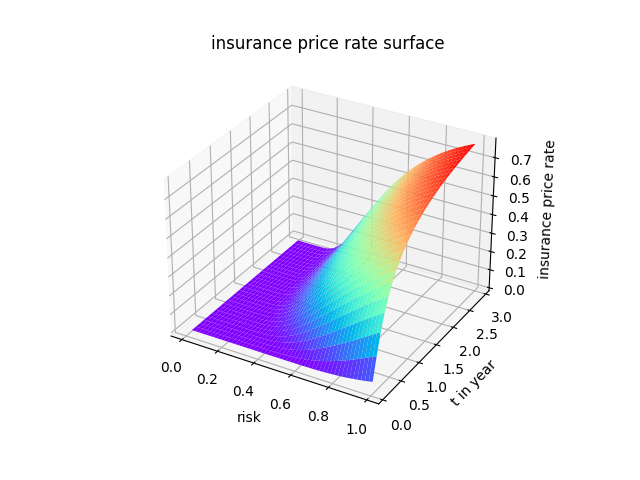
\includegraphics[width=\linewidth]{./graphs/insurance_price_rate_surface} % Figure image
	\caption{Price Changes with the Risk and Expiry Time} % Figure caption
	\label{fig:surface} % Label for referencing with \ref{bear}
\end{figure}

On the surface, the insurance price remains relatively low when the risk is less than 0.4, but it rapidly increases when the risk exceeds 0.4 and the expiry time reaches one year.
When the risk is close to 1.0, it signifies that people have lost faith in this DeFi protocol, and if you buy 100USDT coverage for three years, you will pay more than 70USDT.

\section{Epoch Management}\label{sec:epoch-management}
The introduction of an epoch breaks up the continuous timeline so that the impact of every deposit, withdrawal, and policy purchase is recorded in the specific epoch.
We can easily calculate how much is locked and how much can be withdrawn by epoch calculation.

\subsection{Locked Asset Per Share}\label{subsec:locked-asset-per-share}

The coverage of each policy locked the assets given by all underwriters by their proportion.
When a new policy is sold with the coverage of $C$, the locked asset per share is calculated as follows:

\begin{equation}
	\Delta L = \frac{C}{total\,liquidity}\label{eq:equation2}
\end{equation}

\subsection{Epoch}\label{subsec:epoch}

An epoch is a period of time during which the net $\Delta L$ is calculated and the net $\Delta L$ is the sum of the $\Delta L$ \textbf{before} this epoch minus the $\Delta L$ that has already been settled among them.

\begin{figure}[H]
	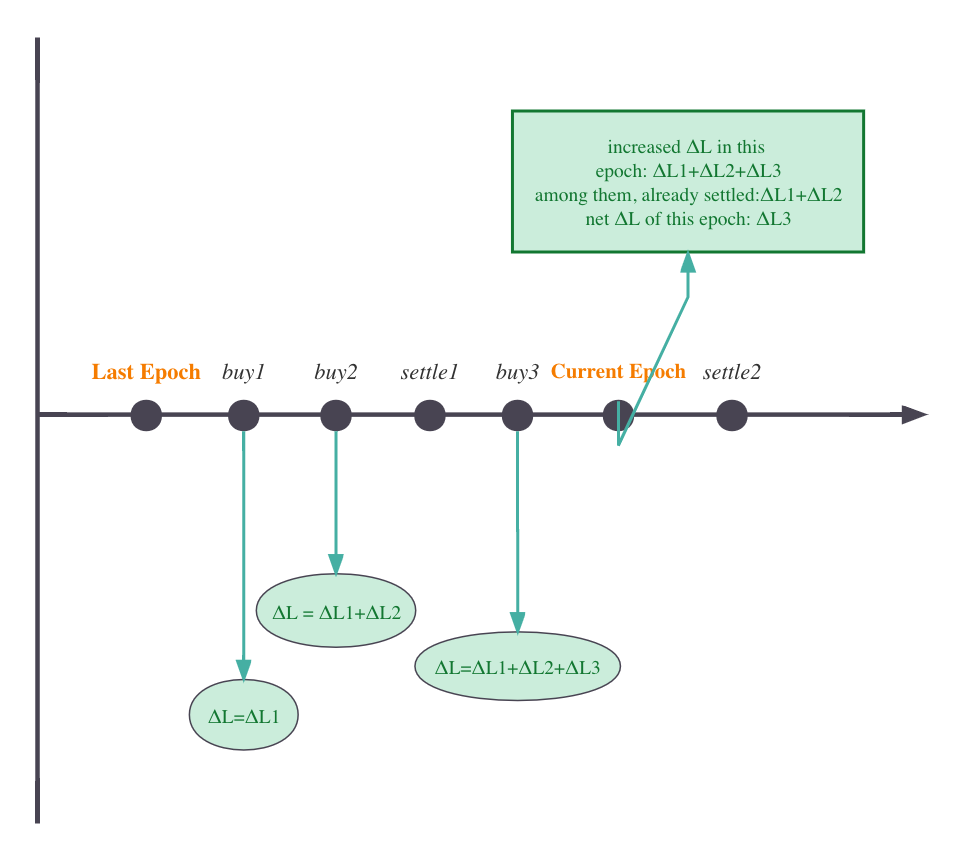
\includegraphics[width=0.8\linewidth]{net_delta_impact}
	\centering
	\caption{Epoch and Net $\Delta L$ calculation} % Figure caption
	\label{fig:epoch-and-net-delta-l} % Label for referencing with \ref{bear}
\end{figure}

The most important parameter in the epoch is the net $\Delta L$.
The epoch will also include some other parameters, such as an index and a start time.

The $\Delta L$ of a certain epoch simply indicates how much asset per share has been locked since the first epoch.
If the underwriter provide the liquidity($l$) at the epoch $i$ and exit at the epoch $j$, the locked asset($L$) can be calculated as follows:

\begin{equation}
	L = l(net \Delta L_{j} - net \Delta L_{i})\label{eq:equation3}
\end{equation}

A certain underwriter's withdrawal asset($W$) will be computed as follows:

\begin{equation}
	W = l - L  = l(1- net \Delta L_{j} + net \Delta L_{i}))\label{eq:equation4}
\end{equation}

With the equation of [\ref{eq:equation3}] and [\ref{eq:equation4}], we can easily calculate the locked asset and the withdrawal asset of each underwriter.
In this case, the underwriter can withdraw the asset at any time without a lock-up period.


\section{Risk Reserve}\label{sec:risk-reserve}
DeFi insurance methods must provide the underwriters with a rate of return equivalent to market alternatives.
Payouts are infrequent with insurance capital, whether underwritten or not, and the capital sits dormant for the most of the time.
To maximize underwriter returns, we will invest a portion of the latent insurance funds in low-risk DeFi portfolios while keeping a payout reserve.
The majority of the earnings on these investments will go to the underwriters, with the rest of them going to the risk reserve.

Risk reserve acts as a buffer in the protocol by collecting some of the mining rewards.
When the risk reserve is sufficient to cover the claim amount, it will pay the policyholder directly rather than using capital from the main pool.


\section{DAO}\label{sec:dao}
Meta Defender has assembled a team of experienced insurance specialists, including actuaries and financial analysts, to provide fair, open, objective, and transparent opinions and claims evaluations.
When a policyholder files a claim, the protocol will thoroughly analyze the opinions of both expert evaluators and community members before deciding whether and how to pay the claim.
Similarly, when the protocol needs a vote on whether to introduce a new insurance program, it will consider both parties' perspectives.
In the future, Meta Defender token hodlers will find more diverse applications in more DeFi scenarios.

%----------------------------------------------------------------------------------------
%	BIBLIOGRAPHY
%----------------------------------------------------------------------------------------
\printbibliography[title={Bibliography}] % Print the bibliography, section title in curly brackets
\begin{thebibliography}{99} % Bibliography - this is intentionally simple in this template
\bibitem[Marcus, Alan and Shaked, Israel, 1984]{Marcus et al., 1984}
Marcus, Alan and Shaked, Israel.
(1984).
\newblock The Valuation of FDIC Deposit Insurance Using Option-pricing Estimates
\newblock {\em Journal of Money, Credit and Banking}, 16:446--60.
\bibitem[RONN, EHUD I. and VERMA, AVINASH K.]{RONN et al., 1986}
RONN, EHUD I. and VERMA, AVINASH K.
(1986).
\newblock Pricing Risk-Adjusted Deposit Insurance: An Option-Based Model
\newblock {\em Journal of Money, Credit and Banking}, 41:871--895.
\bibitem[Laeven and Luc]{Laeven et al., 2002}
Laeven, Luc.
(2002).
\newblock Bank Risk and Deposit Insurance
\newblock {\em The World Bank Economic Review}, 16:109--137.
\bibitem[Falkenheim, Michael and Pennacchi, George]{Falkenheim et al., 2003}
Falkenheim, Michael and Pennacchi, George.
(2003).
\newblock The cost of deposit insurance for privately held banks: A market comparable approach
\newblock {\em Journal of Financial Services Research}, 24:121--148.
\end{thebibliography}

%----------------------------------------------------------------------------------------

\end{document}
